% Automata Course. Challenge Problem #1
\documentclass[preview,11pt]{standalone}
\usepackage[svgnames]{xcolor}
\usepackage{tikz}
\usetikzlibrary{automata,arrows,positioning,fit,calc}
\begin{document}
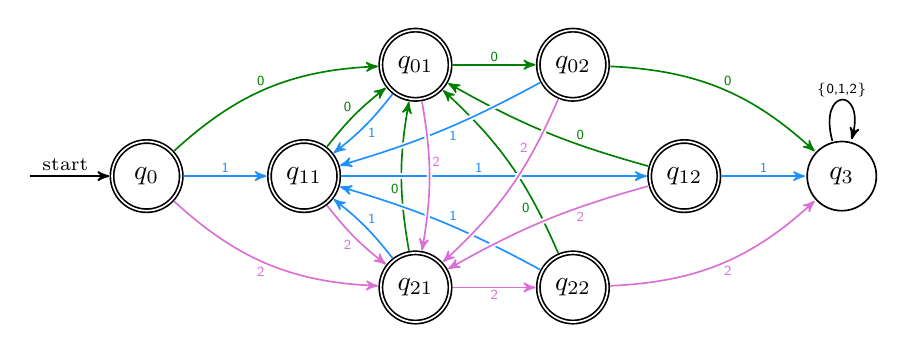
\begin{tikzpicture}[
  on grid,
  ->, >=stealth',shorten <=0.4pt,shorten >=0.5pt,auto,
  node distance=2cm,
  semithick,
  every edge/.append style={font=\sffamily\tiny,inner sep=0.85pt}
  ]

  \node[state,initial text={},accepting] (q_0)                        {$q_0$};
  \node[state,accepting]         (q_11) [right=of q_0]        {$q_{11}$};
  \node[state,accepting]         (q_01) [above right=of q_11] {$q_{01}$};
  \node[state,accepting]         (q_21) [below right=of q_11] {$q_{21}$};
  \node[state,accepting]         (q_02) [right=of q_01]       {$q_{02}$};
  \node[state,accepting]         (q_22) [right=of q_21]       {$q_{22}$};
  \node[state,accepting]         (q_12) [below right=of q_02] {$q_{12}$};
  \node[state]                   (q_3)  [right=of q_12]       {$q_3$};

  \draw[<-,every node/.style={font=\scriptsize,inner sep=1.75pt}]
    (q_0) -- node[above,pos=0.55] {start} ++(-1.5cm,0)
    ;

  \path[->,Green,every node/.style={Green}] 
    (q_0)  edge [bend left=20]  node                      {0}  (q_01)
    (q_01) edge                 node                      {0}  (q_02)
    (q_11) edge [bend left=7]   node                      {0}  (q_01)
    (q_21) edge [bend left=10]  node [pos=0.41]           {0}  (q_01)
    (q_02) edge [bend left=20]  node                      {0}  (q_3)
    (q_12) edge [bend left=7]   node [swap,pos=0.35]      {0}  (q_01)
    (q_22) edge [bend right=12] node [pos=0.28]           {0}  (q_01)
    ;

  \path[->,DodgerBlue,every node/.style={DodgerBlue}] 
    (q_0)  edge                 node                      {1}  (q_11)
    (q_01) edge [bend left=7]   node                      {1}  (q_11)
    (q_11) edge [line width=2pt,draw=White]                    (q_12)
           edge                 node [pos=0.45]           {1}  (q_12)
    (q_21) edge [bend right=7]  node [swap]               {1}  (q_11)

    (q_02) edge [bend left=6,line width=2pt,draw=White]        (q_11)
           edge [bend left=6]   node [pos=0.48]           {1}  (q_11)
    (q_12) edge                 node                      {1}  (q_3)
    (q_22) edge [bend right=6,line width=2pt,draw=White]       (q_11)
           edge [bend right=6]  node [swap,pos=0.48]      {1}  (q_11)
    ;

  \path[->,Orchid,every node/.style={Orchid}] 
    (q_0)  edge [bend right=20] node [swap]               {2}  (q_21)
    (q_01) edge [bend left=10,line width=2pt,draw=White]       (q_21)
           edge [bend left=10]  node [pos=0.40]           {2}  (q_21)
    (q_11) edge [bend right=7]  node [swap]               {2}  (q_21)
    (q_21) edge                 node [swap]               {2}  (q_22)
    (q_02) edge [bend left=12,line width=2pt,draw=White]       (q_21)
           edge [bend left=12]  node [swap,pos=0.30]      {2}  (q_21)
    (q_12) edge [bend right=7,line width=2pt,draw=White]       (q_21)
           edge [bend right=7]  node [pos=0.35]           {2}  (q_21)
    (q_22) edge [bend right=20] node [swap]               {2}  (q_3)
    ;

  \path[->]
    (q_3)  edge [loop above]    node              {\{0,1,2\}}  (q_02)
    ;
\end{tikzpicture}
\end{document}
